\documentclass[a4paper, 10pt]{article}

\usepackage[margin=1in, bottom=1in]{geometry}
\usepackage{setspace}
\usepackage{graphicx}
\usepackage{enumitem}
\usepackage{fancyvrb}
\usepackage{lipsum}
\usepackage{kotex}
\usepackage{subcaption}
\usepackage{xcolor}

\setlist[itemize]{noitemsep}
\setlist[enumerate]{noitemsep}
\setstretch{1.25}

\title{네트워크 소켓 프로그래밍 - 온라인 오목 보고서}
\author{컴퓨터공학부 2016-15523 송우성}
%\date{}

\begin{document}

\maketitle

\section{Problem Statement}
온라인 오목 게임을 만들었다. 각 클라이언트는 접속 시 유일한 플레이어 ID 값을
가진다. 로그인 후, 클라이언트는 게임을 할 수 있는 방을 검색하고, 접속하거나, 새로
생성할 수 있다. 게임 방도 각각 유일한 방 ID를 가진다. 최대 두 명의 플레이어가 방에 접속할
수 있으며, 단 한 명의 플레이어도 방에 접속하지 않은 경우, 그 방은 없어진다. 한
명의 플레이어가 있는 방을 대기(wait) 방이라고 하며, 두 명이 있는 것을 꽉찬(full)
방이라고 한다.

각 방에서 플레이어는 준비(ready)를 하거나 취소할 수 있다. 모든 플레이어는 같은
방에 있는 다른 플레이어의 준비 상태를 실시간으로 확인할 수 있다. 꽉찬 방의 두
플레이어가 모두 준비를 하면 오목 게임을 시작한다. 처음 방에 들어온 플레이어가
선수(흑돌)를 잡으며, 나중에 들어온 플레이어가 후수(백돌)를 잡는다.

게임 화면에서 11x11 크기의 오목판이 주어진다. 각 플레이어는 자신의 차례에
60초 안에 돌을 놓아야한다. 연속으로 5개의 같은 색 돌이 있거나, 상대방의
인터넷 연결이 10초 이상 끊어진 경우 플레이어는 승리한다. 만약 돌을 놓는 시간
제한을 놓치거나, 보드 밖에 돌을 2번 이상 둘 경우 곧바로 패배한다. 두 플레이어가
보드에 놓은 돌의 총 개수가 50개 이상인 경우 무승부로 간주한다. 게임의 승자
상태가 결정되는 순간 결과 화면은 5초 동안 보여지며, 이후 두 플레이어는
게임 대기 방 화면으로 돌아간다.

\section{User Manual}
\subsection{Compilation \& Execution}
우선 \texttt{make}, \texttt{java}가 설치되어있는 환경에서만 실행할 수 있다.
첨부된 파일에는 이미 서버(\texttt{server.java})와 클라이언트(\texttt{client.java})가
모두 컴파일되어있다. 만약 이 두 파일이 없다면,
\begin{Verbatim}[tabsize=4,xleftmargin=2em]
$ make
\end{Verbatim}
명령어를 통해 새로 생성해야한다. 이후, \texttt{configure.xml} 파일을 수정하여
서버의 호스트 주소와 포트 번호를 수정할 수 있다.(기본값으로 서버 호스트는
\texttt{cn1.snucse.org}로 설정되어있다.) 해당 호스트를 접속하여
\begin{Verbatim}[tabsize=4,xleftmargin=2em]
$ java -jar server.jar
\end{Verbatim}
을 통해 콘솔 기반 서버를 실행할 수 있다.

이후 클라이언트는 \texttt{configure.xml} 파일의 내용을 서버의 것과
같게 만들어준 뒤,
\begin{Verbatim}[tabsize=4,xleftmargin=2em]
$ java -jar client.jar
\end{Verbatim}
을 통해 GUI 기반 프로그램을 실행할 수 있다. 만약 \texttt{.jar} 확장자
파일에 대한 기본 프로그램을 JDK Platform Binary로 설정해놓는다면,
아이콘을 더블 클릭하여 클라이언트 프로그램을 실행할 수 있다. 단, 서버와
클라이언트 \texttt{.jar} 파일을 다른 곳으로 옮긴다면 실행이 되지 않는다.

\subsection{Client Manual}
클라이언트 프로그램을 실행했을 때, 서버와 성공적으로 연결이 되면 아래와 같이
플레이어 ID를 생성할 수 있는 화면이 나온다.
보이는 텍스트 필드에 2글자 이상, 20글자 이하의 영문 플레이어 ID를 입력하고
엔터키를 누르거나 Confirm 버튼을 누르면 로그인할 수 있다. 만약 접속 중인
중복된 ID가 이미 있다면, 다시 시도해야한다.
\begin{figure}[h]
  \centering
  \begin{subfigure}{.3\textwidth}
    \centering
    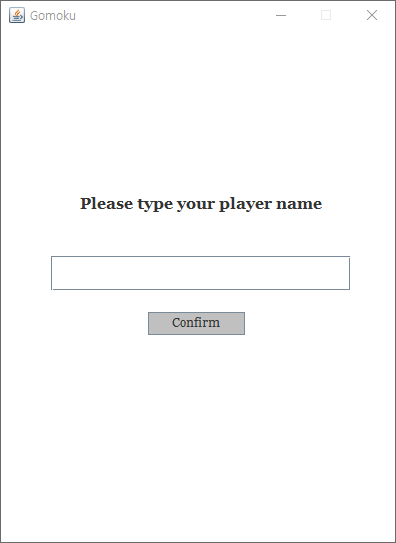
\includegraphics[width=.9\linewidth]{resource/login}
    \caption{플레이어 ID 입력 화면}
    \label{fig:login}
  \end{subfigure}
  \begin{subfigure}{.3\textwidth}
    \centering
    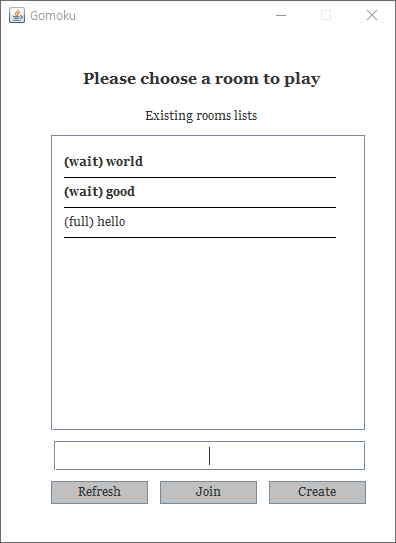
\includegraphics[width=.9\linewidth]{resource/room_search}
    \caption{게임 방을 고르는 화면}
    \label{fig:room_search}
  \end{subfigure}
  \caption{처음 접속할 때 보이는 화면들}
\end{figure}

플레이어 ID를 성공적으로 생성하고나면 접속할 방을 고르는 화면이 나온다.
Refresh 버튼을 누르면 방 리스트를 다시 서버에서 받아온다. 이 버튼을 누르지
않더라도 방 정보가 바뀐 것이 있다면 자동으로 새로고침한다. (wait) 접두어로
된 방은 한 명의 플레이어만 접속하고 있는 곳으로, 접속이 가능하다. (full)
접두어는 두 명의 플레이어가 있는 방으로 접속이 불가능하다. 리스트 안의
방 라벨을 누르면 아래 텍스트 필드에 해당 방의 이름이 채워진다. 텍스트 필드를
채운 뒤 Join 버튼을 누르면 해당 방에 접속 시도를 할 수 있다. 새로운 방을
만들고자하면 텍스트 필드에 2글자 이상, 20글자 이하 영문 방 이름을 넣고
Create 버튼을 누르면 생성할 수 있다. 물론 중복은 허용하지 않는다.

방에 접속하고 나면 아래와 같은 화면이 보인다. 상대 플레이어가 아직 들어오지
않는다면 (Waiting) 라벨이 보인다. 상대 플레이어가 들어오면 그 ID가 보인다.
Ready 버튼을 통해 준비할 수 있고, Cancel 버튼으로 준비를 취소할 수 있다.
Leave 버튼을 누르면 방을 나가서 다시 Figure \ref{fig:room_search} 화면으로
돌아간다. 두 플레이어가 모두 준비 상태이면 게임이 시작된다.
\begin{figure}[h]
  \centering
  \begin{subfigure}{.3\textwidth}
    \centering
    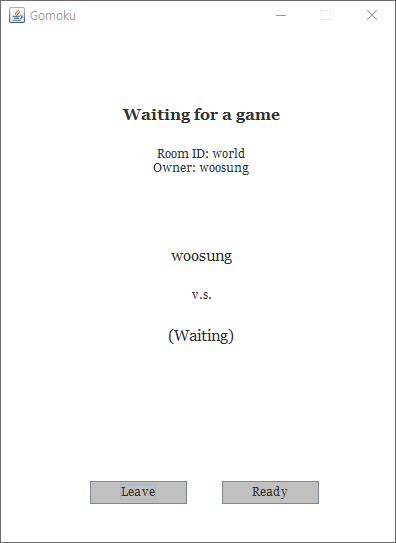
\includegraphics[width=.9\linewidth]{resource/waiting}
    \caption{상대 플레이어가 없을 때}
    \label{fig:waiting}
  \end{subfigure}
  \begin{subfigure}{.3\textwidth}
    \centering
    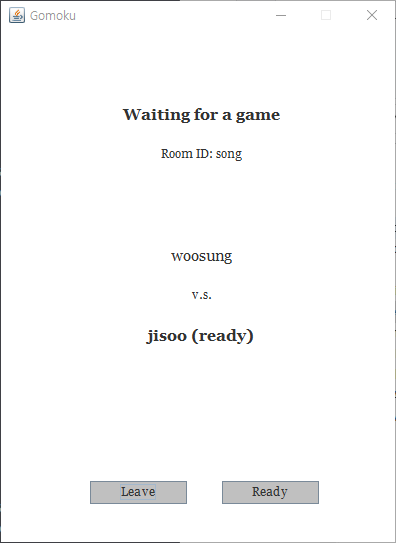
\includegraphics[width=.9\linewidth]{resource/room}
    \caption{상대방이 들어와서 준비를 함}
    \label{fig:room}
  \end{subfigure}
  \caption{게임 방 대기 화면들}
\end{figure}
\newpage

게임이 시작되면 상단에 누구의 차례인지 표기가 되며, 각 차례에 놓는 돌을
색깔도 굵게 표시된다. 각 차례마다 플레이어에게 남은 고민할 시간이 중앙에
초단위로 실시간으로 표시된다. 중복된 위치에 돌을 놓거나, 보드 밖에 돌을
놓는 경우 붉은 색으로 경고 문구가 드러난다. 한 플레이어가 연속된 5개의
돌을 놓으면 승리 화면이 5초 동안 나온다. 그런 뒤 다시 대기 방 화면으로 돌아간다.
\begin{figure}[h]
  \centering
  \begin{subfigure}{.3\textwidth}
    \centering
    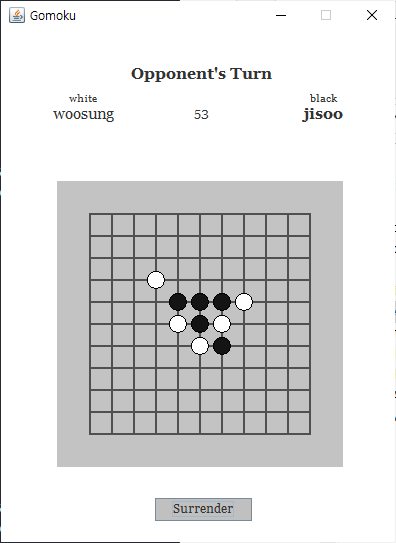
\includegraphics[width=.9\linewidth]{resource/game}
    \caption{누구 차례, 어느 색깔인지 안내}
    \label{fig:waiting}
  \end{subfigure}
  \begin{subfigure}{.3\textwidth}
    \centering
    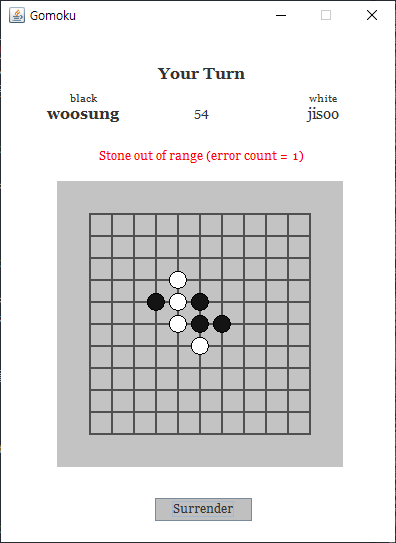
\includegraphics[width=.9\linewidth]{resource/out_of_board}
    \caption{허용되지 않는 동작 경고 문구}
    \label{fig:room}
  \end{subfigure}
  \begin{subfigure}{.3\textwidth}
    \centering
    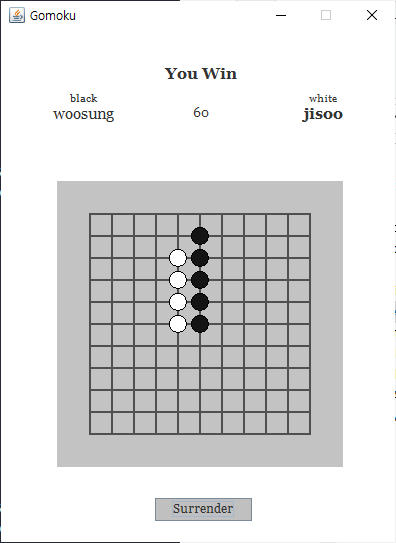
\includegraphics[width=.9\linewidth]{resource/win}
    \caption{흑돌 승리!}
    \label{fig:room}
  \end{subfigure}
  \caption{게임 플레이 화면들}
\end{figure}

\section{Details of Implementation}
\subsection{Development Environment}
우선 Java 오라클 JDK 15 버전이 설치되어있는 윈도우 PC에서 Eclipse IDE
개발환경을 가지고 기본적인 코드를 작성하였다. 그런 뒤, OpenJDK 11 버전이
설치된 리눅스 서버 PC의 Vim 환경에서 디버깅 및 코드 클리닝을 마쳤다.
배포의 편의성을 위해 별도의 외부 라이브러리는 사용하지 않고, pure JAVA로만
개발하였다.

\subsection{Protocol}
서버는 비동기(asynchronous)적으로 여러 클라이언트 처리 쓰레드를 관리하도록
만들었다. 메인 서버는 그저 bind 및 accept만 진행하고, 새로운 소켓 연결이
생성될 때마다 처리 쓰레드를 새로 만들어 실행하는 역할만 수행한다.
기본적으로 서버 쓰레드와 클라이언트는 줄 단위로 짧은 길이의 문자열을 주고받는
통신을 한다. 서버가 클라이언트에게 보내는 문자열의 종류는 플레이어 신호,
상대(opponent) 신호, 그리고 연결 체크(connection check) 신호로 세 종류이다.
클라이언트가 서버에게 보내는 문자열의 종류는 플레이어 신호, 연결 체크(connection
check) 신호로 두 종류이다.

\subsubsection{Connection Check Signal}
서버와 클라이언트는 1초 당 한 번 간격으로 \texttt{connection check}
이라고 불리는 연결 체크 신호를 주고 받는다. 클라이언트 PC의 네트워크가
끊어질 경우 게임이 즉시 중단되는 것이, 60초의 시간 제한만큼 기다리는 것보다
상대 플레이어에게 더 낫다. 그러므로 각 클라이언트가 서버와 연결이 지속적으로
이루어지는지 확인하는 것이 좋다. 만약 이 연결 체크 신호가 10초 동안 감지되지
않는다면, 서버는 클라이언트가 접속이 끊어졌다고 간주하고 관리 쓰레드를 삭제한다.

\subsubsection{Player Signal}
플레이어 신호는 클라이언트 플레이어 그 자체에 대한 정보를 주고받는 데 사용한다.
각 상태에서 클라이언트가 서버에게 보내는 신호의 종류는 아래와 같다.
\begin{itemize}
  \item 로그인 화면에서 보내는 신호
  \begin{itemize}
    \item \texttt{player\\\{playerID\}}: \texttt{\{playerID\}} 이름의 새로운 플레이어를 생성한다.
    \item \texttt{close}: 클라이언트 연결 해제를 서버에게 통보한다.
  \end{itemize}
  \item 게임 방 검색 화면에서 보내는 신호
  \begin{itemize}
    \item \texttt{search}: 서버에게 모든 방의 정보를 가져올 것을 요청한다.
    \item \texttt{join\\\{roomID\}}: \texttt{\{roomID\}} 이름의 방에 접속할 것을 요청한다.
    \item \texttt{create\\\{roomID\}}: \texttt{\{roomID\}} 이름의 방을 생성하고 접속할 것을 요청한다.
    \item \texttt{close}: 클라이언트 연결 해제를 서버에게 통보한다.
  \end{itemize}
  \item 게임 방 안에서 보내는 신호
  \begin{itemize}
    \item \texttt{ready}: 게임 준비가 되었음을 통보한다.
    \item \texttt{cancel}: 게임 준비 해제를 통보한다.
    \item \texttt{leave}: 게임 방에서 나갈 것을 통보한다.
    \item \texttt{close}: 클라이언트 연결 해제를 서버에게 통보한다.
  \end{itemize}
  \item 게임 화면에서 보내는 신호
  \begin{itemize}
    \item \texttt{stone\\\{row\} \{column\}}: \texttt{\{row\}}행 \texttt{\{column\}}열에 자신의 돌을 놓을 것을 요청한다.
    \item \texttt{surrender}: 게임 항복을 서버에게 통보한다.
    \item \texttt{close}: 클라이언트 연결 해제를 서버에게 통보한다.
  \end{itemize}
\end{itemize}

서버가 클라이언트에게 보내는 플레이어 신호는, 클라이언트로부터 온 요청의 응답이거나,
아니면 클라이언트의 상태가 바뀌었음을(예를 들어 게임의 시작) 알려주는 통보이다.
또한, 서버의 부하를 줄이기 위하여 클라이언트가 2분 이상 동작(질의 신호)이 없는 경우
\texttt{query timeout}이라는 신호를 보내어 연결이 끊어졌음을 통보한다.
\begin{itemize}
  \item 로그인 화면에서 보내는 신호
  \begin{itemize}
    \item \texttt{success}: 플레이어 ID 생성 질의가 들어왔을 때, 성공적이었음을 알려준다.
    \item \texttt{fail}: 플레이어 ID 생성 쿼리가 들어왔을 때, 실패했음을 알려준다.
    \item \texttt{invalid}: 상황에 맞지 않는 질의가 들어왔을 때 보낸다.
    \item \texttt{query timeout}: 클라이언트가 질의를 오랫동안(2분) 보내지 않았을 때 연결 해제를 통보한다.
  \end{itemize}
  \item 게임 방 검색 화면에서 보내는 신호
  \begin{itemize}
    \item \texttt{success}: 클라이언트가 요청한 질의를 성공적으로 수행했을 때(할 수 있을 때) 보낸다.
    \begin{itemize}
      \item 만약 \texttt{search} 질의가 왔다면 아래 양식으로 응답한다.
        \begin{Verbatim}[tabsize=4,xleftmargin=2em]
success
{number of rooms}
(wait) {roomID 1}
(wait) {roomID 2}
...
(full) {roomID 1}
(full) {roomID 2}
...
        \end{Verbatim}
        두 번째 줄에 방의 총 개수를 정수로 보낸 뒤, 그 다음 줄부터 방의 세부 정보를 모두 보낸다.
        특히, 대기(wait) 방을 꽉찬(full) 방보다 먼저 리스팅하여 보낸다.
      \item \texttt{join}, \texttt{create} 쿼리에 대해서는 성공적이면 보낸다.
    \end{itemize}
    \item \texttt{fail}: 방 합류나 생성에 문제가 있으면 보낸다.
    \item \texttt{change}: 방 정보에 변경 사항이 있다면 클라이언트에게 보내어 \texttt{search} 질의를 보내게 만든다.
    \item \texttt{invalid}: 상황에 맞지 않는 질의가 들어왔을 때 보낸다.
    \item \texttt{query timeout}: 클라이언트가 질의를 오랫동안(2분) 보내지 않았을 때 연결 해제를 통보한다.
  \end{itemize}
  \item 게임 방 안에서 보내는 신호
  \begin{itemize}
    \item \texttt{success}: 준비, 취소, 나가기 질의가 성공적이면 보낸다.
    \item \texttt{play\\\{turn info\}}: 두 클라이언트가 모두 준비하여 게임이 시작하는 순간에 보낸다.
    \begin{itemize}
      \item \texttt{\{turn info\}}으로 가능한 문자열은 \texttt{your turn}과 \texttt{not your turn}이 있다.
    \end{itemize}
    \item \texttt{invalid}: 상황에 맞지 않는 질의가 들어왔을 때 보낸다.
    \item \texttt{query timeout}: 클라이언트가 질의를 오랫동안(2분) 보내지 않았을 때 연결 해제를 통보한다.
  \end{itemize}
  \item 게임 화면에서 보내는 신호
  \begin{itemize}
    \item \texttt{success}: 돌 놓기, 항복, 나가기 질의가 성공적이면 보낸다.
    \item \texttt{invalid move\\\{reason\}}: 돌 놓기 질의가 실패하면 보낸다.
    \begin{itemize}
      \item \texttt{\{reason\}}으로 가능한 문자열은 \texttt{Stone already on that position}과\\
      \texttt{Stone out of range (error count = 1 or 2)}가 있다.
    \end{itemize}
    \item \texttt{your turn}: 차례가 바뀌어 클라이언트의 순서이면 보낸다.
    \item \texttt{not your turn}: 차례가 바뀌어 클라이언트의 순서가 아니면 보낸다.
    \item \texttt{stone timeout}: 클라이언트가 60초 동안 돌을 놓지 않으면 보낸다.
    \item \texttt{end\\\{result\}}: 게임 종료 시 보낸다.
    \begin{itemize}
      \item \texttt{\{result\}}으로 가능한 문자열은 \texttt{you win}, \texttt{you lose}, \texttt{you draw}가 있다.
    \end{itemize}
    \item \texttt{invalid}: 상황에 맞지 않는 질의가 들어왔을 때 보낸다.
    \item \texttt{query timeout}: 클라이언트가 질의를 오랫동안(2분) 보내지 않았을 때 연결 해제를 통보한다.
  \end{itemize}
\end{itemize}

\subsubsection{Opponent Signal}
상대 신호는 서버가 상대방 플레이어의 행동 정보를 클라이언트에게 알려주기 위해
사용한다. 예를 들어, 상대방이 보드에 돌을 놓은 경우 플레이어에게도 그 위치를
알려줘야 성공적으로 화면에 보여줄 수 있다. 모두 \texttt{opponent}라는 접두어를
가지고 있어서, 클라이언트는 신호를 분리하여 해석할 수 있다.
각 상태에서 서버가 클라이언트에게 보내는 상대 신호는 아래와 같다.
\begin{itemize}
  \item 게임 방 안에서 보내는 신호
  \begin{itemize}
    \item \texttt{opponent join\\opponent \{opponentID\}}: 새로운 상대가 같은 방에 접속했음을 알려준다.
    \item \texttt{opponent ready}: 상대가 준비 완료임을 알려준다.
    \item \texttt{opponent cancel}: 상대가 준비 취소임을 알려준다.
    \item \texttt{opponent leave}: 상대가 방에서 나갔음을 알려준다.
  \end{itemize}
  \item 게임 화면에서 보내는 신호
  \begin{itemize}
    \item \texttt{opponent stone\\opponent \{row\} \{column\}}: 상대가 보드에 돌을 놓았음을 알려준다.
    \item \texttt{opponent \{put stone error reason\}}: 상대 차례일 때, 보드에 돌을 놓는데 실패했다면 그 이유를 알려준다.
    \item \texttt{opponent surrender}: 상대방이 항복했음을 알려준다.
    \item \texttt{opponent leave}: 상대가 방에서 나갔음을 알려준다. (이 경우 플레이어는 게임에 승리한다.)
  \end{itemize}
\end{itemize}

\subsection{Finite State Machine}
\subsubsection{State of Player, Room and Opponent}
서버와 클라이언트는 각각 특정한 상태를 가진다. 이에 따라 서로 다른 질의와 응답 과정을
거치게 된다.
\begin{itemize}
  \item 플레이어가 가지는 상태 (로그인 이전에는 상태가 없음)
  \begin{itemize}
    \item 게임 방 탐색 상태
    \begin{itemize}
      \item \texttt{SEARCH\_ROOM}: 방을 검색하여 찾고 있는 상태
    \end{itemize}
    \item 게임 방 내부 상태
    \begin{itemize}
      \item \texttt{ENTER\_ROOM}: 방에 막 들어온 상태거나, 준비가 되지 않은 상태
      \item \texttt{READY\_ROOM}: 방에서 준비를 마친 상태
    \end{itemize}
    \item 게임 플레이 상태
    \begin{itemize}
      \item \texttt{MY\_TURN}: 내 플레이어가 돌을 놓을 수 있는 상태
      \item \texttt{NOT\_MY\_TURN}: 상대가 돌을 놓을 수 있는 상태
      \item (클라이언트만 있는 상태) \texttt{TERMINATED}: 게임이 끝나고 5초간 보여지는 상태
    \end{itemize}
    \item (클라이언트만 있는 상태) \texttt{EXIT}: 게임 프로그램을 창을 닫은 상태 (close 질의 대기)
  \end{itemize}
  \item 방이 가지는 상태 (서버에서만 관리함)
  \begin{itemize}
    \item 게임 방 탐색 상태
    \begin{itemize}
      \item \texttt{WAIT\_ROOM}: 플레이어가 한 명 밖에 없는 상태 \textbf{\color{red}(available)}
      \item \texttt{FULL\_ROOM}: 플레이어가 두 명 있지만 게임 대기 중인 상태
      \item \texttt{PLAYING}: 플레이어가 두 명이서 게임 중인 상태 \textbf{\color{red}(playing)}
    \end{itemize}
  \end{itemize}
  \item 상대 플레이어 정보로 가지는 상태 (클라이언트에서만 관리함)
  \begin{itemize}
    \item \texttt{NONE}: 아직 상대 플레이어가 없는 상태
    \item 게임 방 내부 상태
    \begin{itemize}
      \item \texttt{ENTER\_ROOM}: 방에 막 들어온 상태거나, 준비가 되지 않은 상태
      \item \texttt{READY\_ROOM}: 방에서 준비를 마친 상태
    \end{itemize}
    \item 게임 플레이 상태
    \begin{itemize}
      \item \texttt{MY\_TURN}: 상대 플레이어가 돌을 놓을 수 있는 상태
      \item \texttt{NOT\_MY\_TURN}: 내 플레이어가 돌을 놓을 수 있는 상태
      \item \texttt{TERMINATED}: 게임이 끝나고 5초간 보여지는 상태
    \end{itemize}
  \end{itemize}
\end{itemize}

\subsubsection{Input State}
또한 서버와 클라이언트가 주고받는 신호는 비동기적이다. 그러므로 모든 종류의 신호들이
교차하여 들어올 수 있음을 염두해야한다. 예를 들어, \texttt{search} 질의에
응답하는 와중에 갑자기 \texttt{connection check} 신호를 보내야할 수도 있고,
플레이어 신호를 보내는 중에 상대 신호를 보내야할 수도 있다. 이런 경우를 제대로
처리하기 위해 서버와 클라이언트는 모두 들어온 신호를 접두어로 분류하여 처리하는
기능이 있으며, 플레이어와 상대의 상태(State)는 물론, 기대하는 입력 신호의
상태(InputState) 또한 FSM 단위로 관리해야한다.

예를 들어, 클라이언트가 방을 탐색하는 \texttt{search} 신호를 보낸 뒤, 서버에게
기대하는 응답은 여러 줄로 쪼개어져있다. 아래에서 클라이언트는 \texttt{C},
서버는 \texttt{S}로 표기한다.
\begin{Verbatim}[tabsize=4,xleftmargin=2em]
(C -> S) search        - (state, inputState) = (SEARCH_ROOM, OUT_ROOM)
(C <- S) success       - (state, inputState) = (SEARCH_ROOM, SEARCH_ROOM)
(C <- S) 4             - (state, inputState) = (SEARCH_ROOM, SEARCH_ROOM), searchCnt = 4
(C <- S) (wait) room 1 - (state, inputState) = (SEARCH_ROOM, SEARCH_ROOM), searchCnt = 3
(C <- S) (wait) room 2 - (state, inputState) = (SEARCH_ROOM, SEARCH_ROOM), searchCnt = 2
(C <- S) (full) room 3 - (state, inputState) = (SEARCH_ROOM, SEARCH_ROOM), searchCnt = 1
(C <- S) (full) room 4 - (state, inputState) = (SEARCH_ROOM, OUT_ROOM)
\end{Verbatim}
위와 같은 방식으로 클라이언트는 자신의 상태와 기대하는 입력 상태를 둘 다 저장한다.
이를 통해 중간에 비동기적으로 다른 종류의 신호가 들어오더라도 일관성있게
동작할 수 있다.
\begin{Verbatim}[tabsize=4,xleftmargin=2em]
(C -> S) search        - (state, inputState) = (SEARCH_ROOM, OUT_ROOM)
(C <- S) success       - (state, inputState) = (SEARCH_ROOM, SEARCH_ROOM)
(C <- S) 4             - (state, inputState) = (SEARCH_ROOM, SEARCH_ROOM), searchCnt = 4
(C <- S) (wait) room 1 - (state, inputState) = (SEARCH_ROOM, SEARCH_ROOM), searchCnt = 3
(C <- S) connection check - this is not a roomID
(C <- S) (wait) room 2 - (state, inputState) = (SEARCH_ROOM, SEARCH_ROOM), searchCnt = 2
(C <- S) (full) room 3 - (state, inputState) = (SEARCH_ROOM, SEARCH_ROOM), searchCnt = 1
(C <- S) (full) room 4 - (state, inputState) = (SEARCH_ROOM, OUT_ROOM)
\end{Verbatim}
또한, 연결 체크는 \texttt{connection check}로, 상대 신호는 \texttt{opponent}를
접두어로 가지고 있으므로 신호를 분류하여 다르게 상태를 갱신해줄 수 있다.
\begin{Verbatim}[tabsize=4,xleftmargin=2em]
(C -> S) stone
(C -> S) 5 6
(C <- S) success
(C <- S) not your turn
(C <- S) opponent stone
(C <- S) opponent 6 6
(C <- S) your turn
(C -> S) stone
(C -> S) 5 5
(C <- S) opponent surrender - intercept signal from opponent (expect success)
(C <- S) success
(C <- S) end
(C <- S) you win
\end{Verbatim}

결론적으로 모든 신호는 적절한 접두어가 붙어져있으며,
클라이언트는 자기 자신(Player)와 상대(Opponent)에 대한 상태(state)와
기대 입력 상태(inputState)를 모두 저장하기 때문에 비동기적인 입력 신호에도
적절하게 반응할 수 있게 된다. 마찬가지로 서버도 모든 클라이언트 플레이어에
대한 상태(state)와 기대 입력 상태(inputState)를 저장하고 있으므로
연결 체크 신호가 비동기적으로 도착해도 적절하게 처리할 수 있다.
\newpage

\subsection{Modules \& Functions}
소스 코드의 전체적인 구성도는 아래와 같다.
\begin{Verbatim}[tabsize=4,xleftmargin=2em,baselinestretch=1]
src
├── client
│     ├── Client.java
│     ├── Player.java
│     ├── Opponent.java
│     ├── Board.java
│     └── GUI.java
├── graphics
│     ├── PlayerIDFrame.java
│     ├── RoomSelectFrame.java
│     ├── RoomFrame.java
│     └── GameFrame.java
├── gomoku
│     └── Gomoku.java
└── server
       ├── Server.java
       ├── ServerThread.java
       ├── Player.java
       └── Room.java
\end{Verbatim}
아래 부분에서 필수 메소드는 {\color{red} 붉은 색 글씨}로 표기하여 강조하겠다.

\subsubsection{Client Package (\texttt{client})}
클라이언트 실행부이다. 클라이언트는 따로 쓰레드를 관리할 필요가 없으므로
거의 모든 변수와 함수는 static하게 선언되어있다. 각 모듈에 대한 설명과 주요
함수 내용은 아래와 같다.
\begin{itemize}
  \item \texttt{Client.java}
  \begin{itemize}
    \item[] 메인 함수가 위치하는 부분이다. 커다란 \texttt{while} 루프를 돌면서 GUI 유저 입력에 따른 신호를 클라이언트에게 보내고,
    서버에게 받은 신호를 접두어를 통해 FSM들에게 분배한다. 이 루프에서 1초에 한 번씩 연결 체크 신호도 보내며, 10초 동안 서버에게서
    신호가 오지 않으면 네트워크가 끊어진 것으로 간주하고 게임을 종료한다. 정상적으로 게임이 끝난 경우 5초 간 sleep 하는 부분도 여기서 처리한다.
    모든 GUI 프레임을 관리하며, 게임 정보도 관리한다. 질의와 응답을 분류하여 FSM들에게 적절하게 전달하는 머리 부분이다.
    \item \texttt{static void write(String str)}: 서버에게 문자열을 보내는 함수이다.
    \item \texttt{static void pendQuery(String str)}: 서버에게 보낼 문자열을 큐에 집어넣는 함수이다.
    GUI 버튼이 클릭되면 이게 콜 된다. 결국 질의를 보내면서 클라이언트 FSM의 상태를 바꿔야할 수도 있으므로
    큐에 담아두고 처리하는게 낫다.
    \item \texttt{static boolean isQueryPended()}: 큐에 질의가 있는지 확인하는 함수
    \item \texttt{static String nextQuery()}: 다음 쿼리를 찾는 함수. 클라이언트는 큐가 비어있을 때 이 함수를 콜 하지 않는다.
    \item \texttt{static void setConnectionCheckTimer()}: 연결 체크 수신 기준 시각을 지금으로 설정한다.
    \item \texttt{static void setConnectionSendTimer()}: 연결 체크 전송 기준 시각을 지금으로 설정한다.
    \item \texttt{static boolean shouldSendConnectionSend()}: 연결 체크를 서버로 전송한지 1초 이상인지 반환하는 함수다.
    \item \texttt{static boolean isConnectionCheckTimeout()}: 서버로부터 10초 이상 연결 체크 신호가 안 왔는지 반환한다.
  \end{itemize}
  \item \texttt{Player.java}
  \begin{itemize}
    \item[] 플레이어 자신의 정보를 담고 있는 FSM이다.
    \item \texttt{static void processQuery(String query)}: 클라이언트가 서버에게 질의를 보낼 때 FSM의 상태가 바뀌는 경우가 있다. 이를 처리하는 함수이다.
    \item \texttt{static void processResponse(String response)}: 서버로부터 받은 응답에 따라 상태를 변화시키는 함수이다.
  \end{itemize}
  \item \texttt{Opponent.java}
  \begin{itemize}
    \item[] 상대 플레이어 정보를 담고 있는 FSM이다. 서버로부터 받은 신호 중 \texttt{opponent} 접두어가 붙은 것들이 여기서 처리된다.
    \item \texttt{static void processResponse(String response)}: 서버로부터 받은 상대방의 응답에 따라 상태를 변화시키는 함수이다.
  \end{itemize}
  \item \texttt{Board.java}
  \begin{itemize}
    \item[] 클라이언트가 저장하는 게임 보드 정보 저장소이다. 클라이언트는 연속한 5개의 돌, 돌 위치 중복 등
    보드의 의미적인(semantic) 부분을 전혀 계산하지 않고, 서버로부터 그 정보를 통보받기만 한다.
    즉, 이 모듈은 단순히 보드 이차원 배열과 차례 정보, 승자 정보 정도만 담고 있다.
    \item \texttt{void begin(String id1, String id2)}: 선수자와 후수자의 ID 정보를 받고 게임을 초기화하여 시작 준비한다.
  \end{itemize}
  \item \texttt{GUI.java}
  \begin{itemize}
    \item[] 클라이언트가 보는 GUI 화면을 관리하는 함수이다. Player 모듈의 FSM에 따라 서로 다른 화면을 보여주며,
    새로운 화면 정보를 변경해야할 때 적절하게 업데이트해준다.
    \item \texttt{static void repaint()}: Player의 상태에 맞게 새로 화면 정보를 업데이트해준다.
    \item \texttt{static void synchronizeFrameBounds()}: 모든 화면의 위치를 동기화시켜준다.
    \item \texttt{static void showFrame()}: Player의 상태에 맞는 프레임을 적절하게 바꿔서 보여준다.
  \end{itemize}
\end{itemize}

\subsubsection{Client GUI Package (\texttt{graphics})}
클라이언트의 GUI 프레임 정보를 담고있는 패키지이다. 각 모듈에 대한 설명과 주요
함수 내용은 아래와 같다.
\begin{itemize}
  \item \texttt{PlayerIDFrame.java}
  \begin{itemize}
    \item[] 로그인 화면이다. 여기서 플레이어는 자신의 ID를 생성할 수 있다.
    \item \texttt{void setPlayerIDErrorMsg(String errorMsg)}: 플레이어 ID 생성의 응답이 \texttt{fail}일 때, 그 이유를
    화면 상에 보여주는 함수이다.
  \end{itemize}
  \item \texttt{RoomSelectFrame.java}
  \begin{itemize}
    \item[] 로그인 직후 방들을 탐색할 수 있는 화면이다. 방 ID를 직접 입력하거나 버튼으로 입력할 수 있게 텍스트 필드가 있다.
    입력된 방 ID로 접속하는 Join, 새로 생성하는 Create, 혹은 새로고침하는 Refresh 버튼이 위치한다. 
    \item \texttt{void initializeRoomLabels()}: 방 검색 화면을 초기화한다.
    \item \texttt{void addRoomlabel(String roomInfo)}: 방 검색 리스트에 새로운 방 정보를 추가한다.
    해당 라벨이 클릭되면 텍스트 필드에 그 방 ID가 채워지도록 링크한다.
  \end{itemize}
  \item \texttt{RoomFrame.java}
  \begin{itemize}
    \item[] 게임 대기 방을 보여주는 화면이다. 상대방의 ID와 준비 상태를 실시간으로 확인할 수 있다.
    \item \texttt{void setPlayerID(String playerID)}: 플레이어 ID 라벨을 채운다.
    \item \texttt{void setPlayerReadyOrCancel(boolean ready)}: 준비 상태를 바꾼다. Ready 버튼이 Cancel로 바뀌거나 돌아오고,
    준비된 플레이어는 굵은 글씨로 표시된다.
    \item \texttt{void setOpponentID(String playerID)}: 상대방 ID 라벨을 채운다.
    \item \texttt{void setOpponentReadyOrCancel(boolean ready)}: 상대의 준비 상태를 바꾼다.
  \end{itemize}
  \item \texttt{GameFrame.java}
  \begin{itemize}
    \item[] 게임 화면이다.
    \item \texttt{void synchronizeBoard(Board board)}: 게임 보드 이차원 배열으로부터 GUI 정보를 일치화시킨다.
    \item \texttt{void putStone(int row, int column, int turnID)}: 보드의 한 위치만 repaint하여 로드를 줄이는 함수이다.
    \item \texttt{void setPlayerID(String playerID, int playerTurn)}: 플레이어의 ID와 차례 정보를 화면에 갱신하는 함수이다.
    \item \texttt{void setOpponentID(String opponentID, int opponentTurn)}: 상대의 ID와 차례 정보를 화면에 갱신하는 함수이다.
    \item \texttt{void setPlayerTurn()}: 내 플레이어 차례임을 암시해주는 화면으로 갱신한다.
    \item \texttt{void setOpponentTurn()}: 상대 차례임을 암시해주는 화면으로 갱신한다.
  \end{itemize}
\end{itemize}
\begin{figure}[h]
  \centering
  \begin{subfigure}{.24\textwidth}
    \centering
    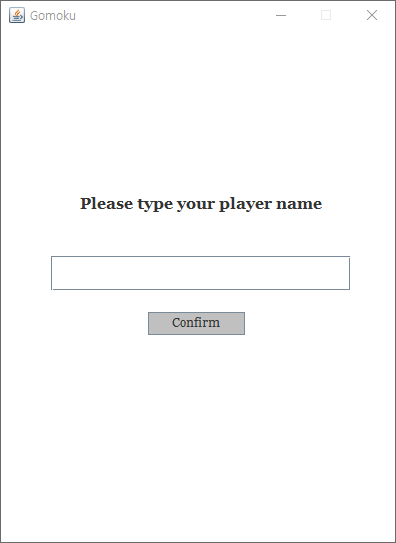
\includegraphics[width=.9\linewidth]{resource/login}
    \caption{PlayerIDFrame}
    \label{fig:player_id_frame}
  \end{subfigure}
  \begin{subfigure}{.24\textwidth}
    \centering
    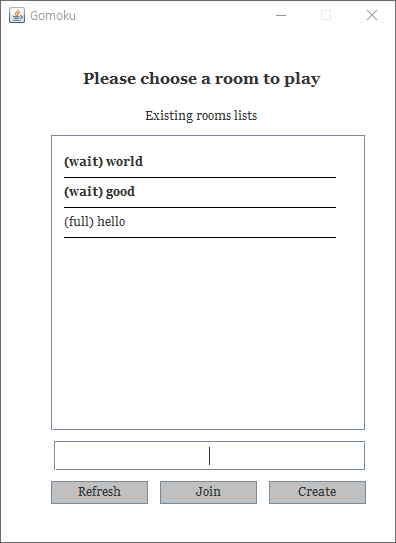
\includegraphics[width=.9\linewidth]{resource/room_search}
    \caption{RoomSelectFrame}
    \label{fig:room_select_frame}
  \end{subfigure}
  \begin{subfigure}{.24\textwidth}
    \centering
    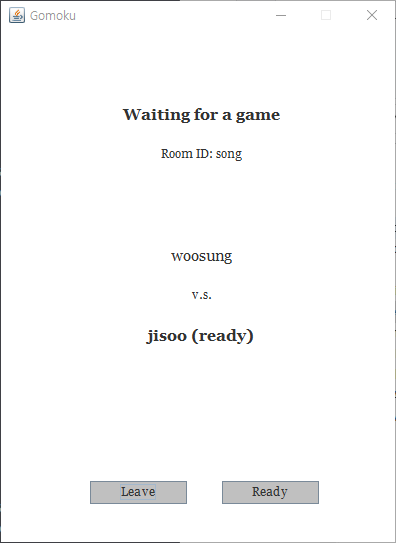
\includegraphics[width=.9\linewidth]{resource/room}
    \caption{RoomFrame}
    \label{fig:room_frame}
  \end{subfigure}
  \begin{subfigure}{.24\textwidth}
    \centering
    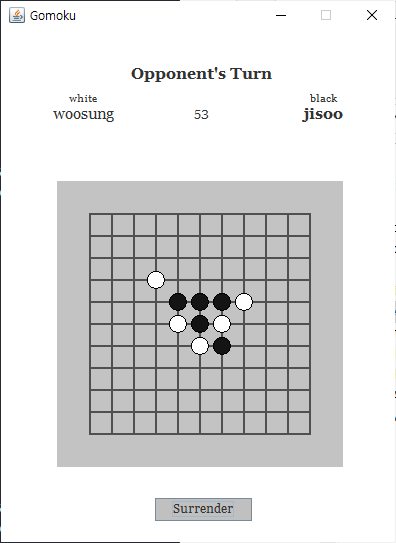
\includegraphics[width=.9\linewidth]{resource/game}
    \caption{GameFrame}
    \label{fig:game_frame}
  \end{subfigure}
  \caption{graphics 패키지 모듈들}
\end{figure}

\subsubsection{Server Game Semantics Package (\texttt{gomoku})}
서버에서 저장하고 해석하는 게임 보드의 정보이다. 클라이언트와 달리 연속된 5개 돌,
보드 밖의 돌, 중복되는 돌 등, 보드의 의미적인(semantic) 계산을 수반한다.
\begin{itemize}
  \item \texttt{Gomoku.java}
  \begin{itemize}
    \item[] 자바로 만든 간단한 오목 프로그램이다. 메인 함수를 통해 CUI 기반 게임을 하여 디버깅하였다.
    \item \texttt{void initialize()}: 보드를 초기화한다.
    \item \texttt{boolean putStone(int row, int column)}: 해당 위치에 돌을 놓을 수 있는지 확인하는 함수이다.
    만약 가능하다면 참 값을 반환하고, 그렇지 않다면 클래스 내 \texttt{putStoneErrorMsg} 문자열을 갱신한 후
    거짓 값을 반환한다. 만약 오목을 만드는 승자가 생기거나, 50수 이상의 돌을 놓거나,
    한 플레이어가 보드 밖에 돌을 두 차례 놓는 상황이 생긴다면 즉시 게임을 종료시킨다.
    \item \texttt{boolean isOutOfRange(int row, int column)}: 해당 위치가 보드 밖인지 감지하는 함수이다.
    \item \texttt{boolean isConsecutiveFive(int row, int column)}: 현 차례의 플레이어가 해당 위치에 돌을
    놓았을 때, 연속된 5개 돌 모양이 생기는지 반환한다.
  \end{itemize}
\end{itemize}

\subsubsection{Server Package (\texttt{server})}
서버가 실행되는 부분이다. 비동기적 서버로써, 새로운 클라이언트를 accept할 때마다
다른 쓰레드를 만든다.
\begin{itemize}
  \item \texttt{Server.java}
  \begin{itemize}
    \item[] 메인 함수가 위치한다. 처음에 \texttt{configure.xml}을 읽어 해당하는 포트에
    서버를 bind시키고, 계속 listen하면서 새로운 클라이언트가 연결되면 ServerThread 하나를
    생성하여 처리하게 시킨다. 존재하는 모든 쓰레드(ServerThread), 플레이어(Player), 방(Room)
    정보를 ArrayList 자료구조로 저장시켜 추가, 검색, 삭제가 용이하게 하였다.
    \item \texttt{static boolean addPlayer(String playerID), {static boolean addRoom(String roomID)}, static void addThread(ServerThread thread)}:
    새로운 플레이어, 방, 쓰레드를 추가한다. 추가가 불가능하면 거짓 값을 반환한다.
    \item \texttt{static Player fetchPlayer(String playerID), static Room fetchRoom(String roomID), static void fetchThread(String playerID)}:
    플레이어, 방, 쓰레드를 검색한다. 존재하지 않는 값이면 null을 반환한다.
    \item \texttt{static boolean erasePlayer(String playerID), static boolean eraseRoom(String roomID), static void eraseThread(ServerThread thread)}:
    플레이어, 방, 쓰레드를 삭제한다.
  \end{itemize}
  \item \texttt{ServerThread.java}
  \begin{itemize}
    \item[] 각 클라이언트와의 교류를 담당하는 쓰레드이다. 클라이언트 플레이어의 상태를 저장하고 있다.
    클라이언트로부터 온 질의에 대해 적절하게 응답해주는 역할을 한다. 타임아웃에 대한 부분도 여기서 관리하며,
    상대방이 있는 경우 \texttt{opponent} 접두어를 붙인 상대 신호를 보낼 수도 있으므로, 상대방의 ServerThread 값을 가지고도 있다.
    \item \texttt{static void write(String str)}: 클라이언트에게 문자열을 보내는 함수이다.
    \item \texttt{static void writeOpponent(String str)}: 상대방 클라이언트에게 \texttt{opponent} 접두어를 붙인 문자열을 보내는 함수이다.
    \item \texttt{static void disconnectMeFromOpponentThread}: 상대방 클라이언트에게 나와 연결이 끊어졌음을 보내는 함수이다.
    \item \texttt{static void setQueryTimer()}: 클라이언트로부터 최근 질의를 받은 시각을 지금으로 설정한다.
    \item \texttt{static void setConnectionCheckTimer()}: 연결 체크 수신 기준 시각을 지금으로 설정한다.
    \item \texttt{static void setConnectionSendTimer()}: 연결 체크 전송 기준 시각을 지금으로 설정한다.
    \item \texttt{static boolean shouldSendConnectionSend()}: 연결 체크를 클라이언트로 전송한지 1초 이상인지 반환하는 함수다.
    \item \texttt{static boolean isThreadTimeout()}: 클라이언트로부터 10초 이상 연결 체크 신호가 안 왔는지, 그리고 질의가 120초 이상 안 왔는지 확인한다.
  \end{itemize}
  \item \texttt{Player.java}
  \begin{itemize}
    \item[] 각 클라이언트의 플레이어 정보와 상태를 저장하는 저장소이다.
    \item \texttt{static boolean isValidPlayerID(String id)}: 2자 이상, 20자 이하 문자열인지 확인한다.
    \item \texttt{\color{red} boolean createAndEnterRoom(String roomID)}: 해당 방을 생성하고 입장하는 함수이다.
    \item \texttt{\color{red} boolean enterRoom(String roomID)}: 해당 방으로 입장하는 함수이다.
    \item \texttt{\color{red} void leaveRoom()}: 원래 있던 방에서 나가는 함수이다.
    \item \texttt{String opponentID()}: 상대 ID를 가져오는 함수이다.
    \item \texttt{\color{red} void ready(), void cancel()}: 게임 대기 방에서 준비 및 취소하는 함수이다.
    \item \texttt{boolean isReadyOrPlaying()}: 본 플레이어가 준비 중이거나, 게임 플레이 중인지 확인하는 함수이다.
    한 방에 있는 모든 플레이어가 동시에 ready에서 playing 상태로 전환하지 않으므로, 이 함수로부터 게임 시작 가능성을
    체크하는 것이 합리적이다.
    \item \texttt{boolean isMyRoomReady()}: 내 방의 모든 플레이어가 준비 완료인지 반환한다.
    \item \texttt{void initializeGame()}: 오목 보드를 초기화하고, 플레이어의 상태를 갱신한다.
    \item \texttt{\color{red} boolean putStone(int row, int column)}: 해당 위치에 돌을 놓는다. 해당 플레이어의
    게임 방 ID는 이미 고정된 상황이므로 PPT 슬라이드처럼 인자로 넣지 않았다.
    \item \texttt{String putStoneErrorMsg()}: 돌을 놓는데 실패했을 때, 그 이유를 가져온다.
    \item \texttt{void setWinner(), void setLoser(), void setDraw()}: 게임의 최종 상태를 결정한다.
    \item \texttt{void setTimer()}: 돌 놓기 60초 제한 시간의 기준점을 지금으로 설정한다.
    \item \texttt{boolean isTimeout()}: 돌 놓기 60초 제한을 넘겼는지 반환한다.
    \item \texttt{boolean isGameTerminated()}: 게임이 끝났는지 반환한다.
    \item \texttt{void endGame()}: 게임을 종료한다.
    \item \texttt{boolean isWinner(), boolean isLoser(), boolean isDraw()}: 게임의 최종 상태를 반환한다.
  \end{itemize}
  \item \texttt{Room.java}
  \begin{itemize}
    \item[] 각 방의 정보와 상태를 저장하는 저장소이다.
    \item \texttt{static boolean isValidRoomID(String id)}: 2자 이상, 20자 이하 문자열인지 확인한다.
    \item \texttt{void addPlayer(Player player)}: 플레이어를 방에 입장시킨다.
    \item \texttt{void removePlayer(Player player)}: 플레이어를 방에서 추방시킨다.
    \item \texttt{boolean isDestructable()}: 방에 플레이어가 아무도 없어 제거할 수 있는지 반환한다.
    \item \texttt{void setTurnsOfPlayers()}: 게임 시작 직전 선수와 후수를 지정한다. 각 방은 플레이어들을
    하나의 ArrayList로 관리하는데, 먼저 방에 접속한 플레이어가 첫 번째 인덱스로 들어가기 때문에 {\color{red} owner ID}가
    잘 정의되며, 그를 항상 선수로 둔다.
    \item \texttt{void initializeGame()}: 오목 보드를 초기화하고, 방 상태를 갱신한다.
    \item \texttt{boolean putStone(int row, int column)}: 해당 위치에 돌을 놓는다.
    \item \texttt{void setWinner(String playerID), void setLoser(String playerID)}: 게임의 최종 상태를 결정한다.
    \item \texttt{void endGame()}: 게임을 종료한다.
  \end{itemize}
\end{itemize}

\section{Results}
사용자 설명에 캡처한 이미지와 같이 기본적인 문제 정의는 모두 정상적으로 실행되었다.
실제로 서버를 실행시킨 뒤 클라이언트 한 명은 내 노트북으로, 다른 한 명은 다른 노트북으로
실행하여 접속했더니 로그인 및 방 생성/접속 과정이 문제없이 수행되었으며,
실시간으로 준비/취소, 돌 놓기, 항복 정보가 전송되어 원할하게 게임할
수 있었다. 연속된 5개를 만들었을 떄 승리 조건이 잘 나타났고, 50개의 돌을 입력했을 때
무승부 표시도 제대로 동작했다.
\begin{figure}[h]
  \centering
  \begin{subfigure}{.3\textwidth}
    \centering
    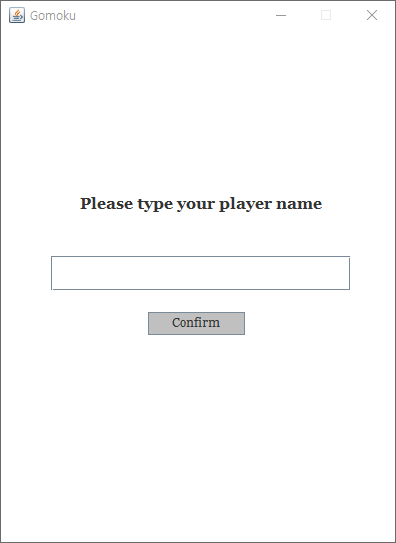
\includegraphics[width=.9\linewidth]{resource/login}
    \caption{플레이어 로그인}
    \label{fig:login}
  \end{subfigure}
  \begin{subfigure}{.3\textwidth}
    \centering
    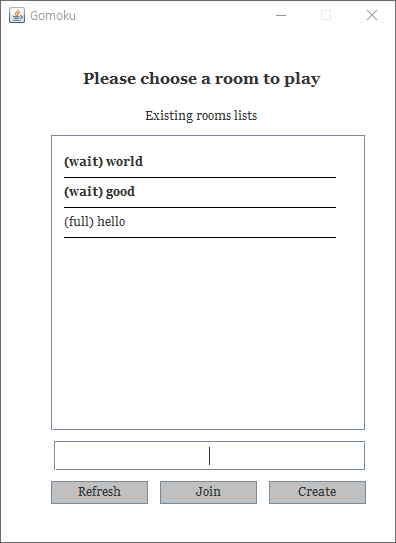
\includegraphics[width=.9\linewidth]{resource/room_search}
    \caption{방 검색 화면}
    \label{fig:room_search}
  \end{subfigure}
  \begin{subfigure}{.3\textwidth}
    \centering
    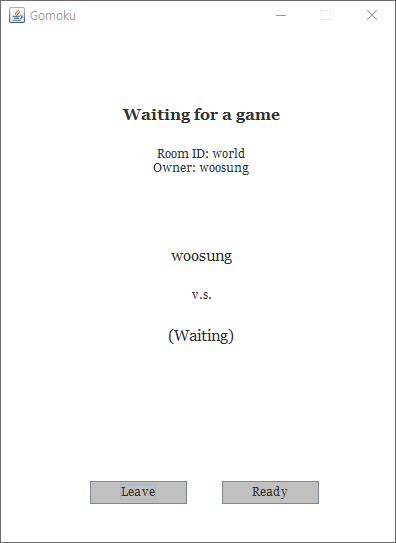
\includegraphics[width=.9\linewidth]{resource/waiting}
    \caption{방 생성 및 접속 직후}
    \label{fig:draw}
  \end{subfigure}
  \caption{게임 접속 결과 화면들}
\end{figure}
\newpage

\begin{figure}[h]
  \centering
  \begin{subfigure}{.3\textwidth}
    \centering
    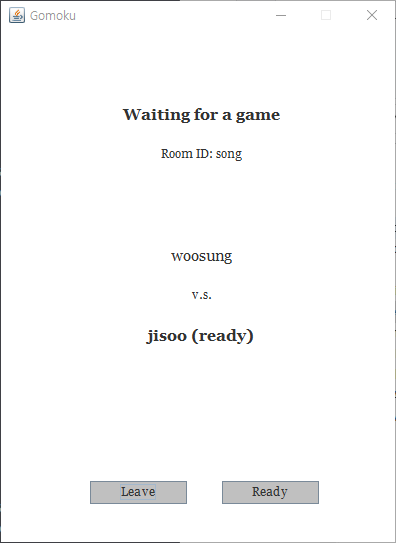
\includegraphics[width=.9\linewidth]{resource/room}
    \caption{실시간 준비 및 취소}
    \label{fig:ready}
  \end{subfigure}
  \begin{subfigure}{.3\textwidth}
    \centering
    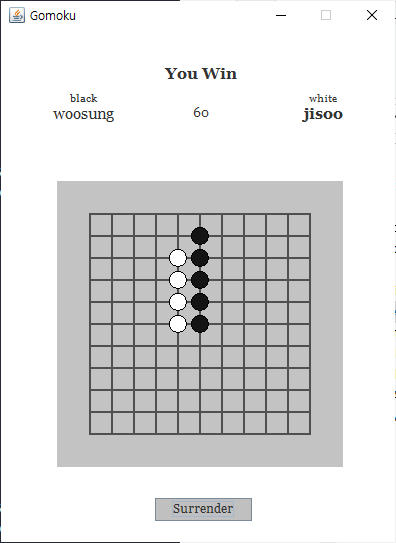
\includegraphics[width=.9\linewidth]{resource/win}
    \caption{오목 승리}
    \label{fig:win}
  \end{subfigure}
  \begin{subfigure}{.3\textwidth}
    \centering
    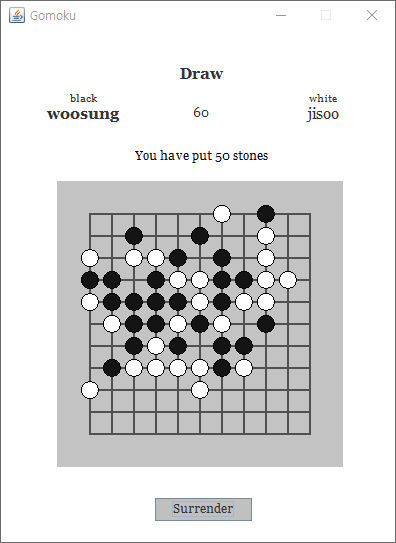
\includegraphics[width=.9\linewidth]{resource/draw}
    \caption{50수 무승부}
    \label{fig:draw}
  \end{subfigure}
  \caption{게임 플레이 결과 화면들}
\end{figure}

요구하는 조건과 맞지 않는 플레이어 ID나 방 ID를 생성하거나, 중복된 ID가 있는
경우 아래와 같이 적절하게 경고창이 나타났다.
\begin{figure}[h]
  \centering
  \begin{subfigure}{.24\textwidth}
    \centering
    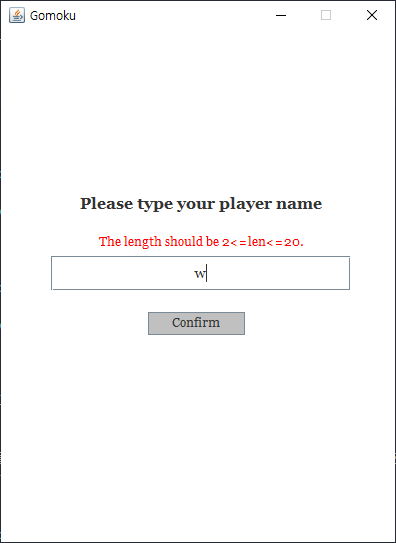
\includegraphics[width=.9\linewidth]{resource/improper_playerID}
    \caption{부적절 플레이어 ID}
    \label{fig:improper_playerID}
  \end{subfigure}
  \begin{subfigure}{.24\textwidth}
    \centering
    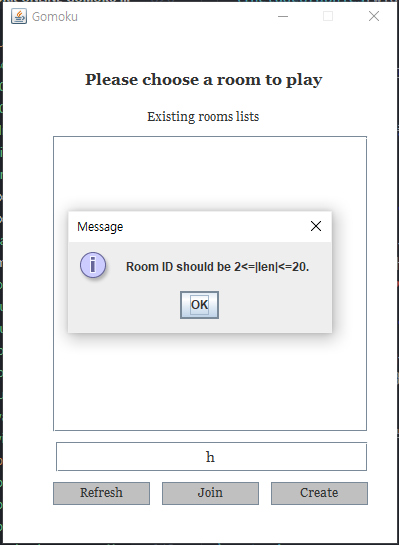
\includegraphics[width=.9\linewidth]{resource/improper_roomID}
    \caption{부적절 방 ID}
    \label{fig:improper_roomID}
  \end{subfigure}
  \begin{subfigure}{.24\textwidth}
    \centering
    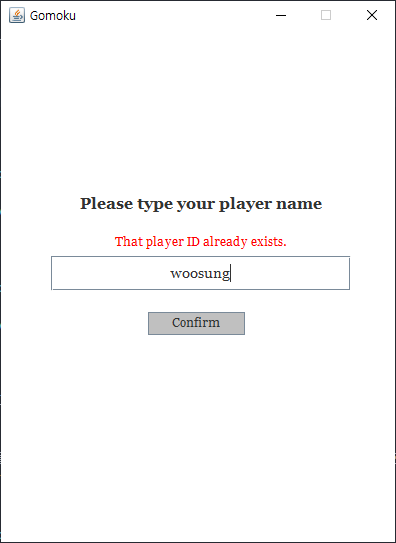
\includegraphics[width=.9\linewidth]{resource/existing_playerID}
    \caption{중복 플레이어 ID}
    \label{fig:existing_playerID}
  \end{subfigure}
  \begin{subfigure}{.24\textwidth}
    \centering
    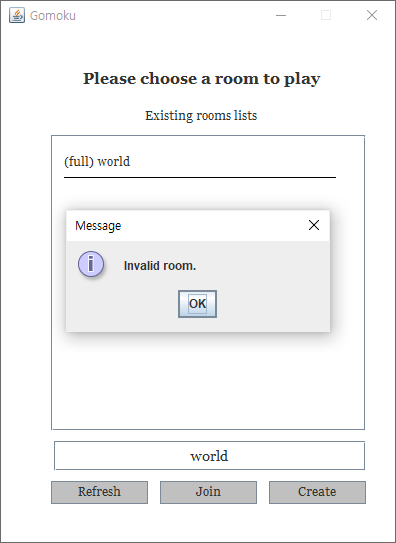
\includegraphics[width=.9\linewidth]{resource/existing_roomID}
    \caption{중복 방 ID}
    \label{fig:existing_roomID}
  \end{subfigure}
  \caption{ID 생성 오류 결과 화면들}
\end{figure}
\newpage

보드 밖 영역에 돌을 놓거나 중복된 위치에 놓고자하는 경우 붉은 색으로 경고창이
적절하게 나타났다.
\begin{figure}[h]
  \centering
  \begin{subfigure}{.3\textwidth}
    \centering
    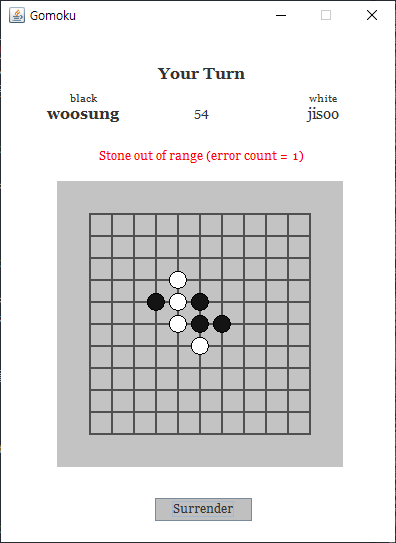
\includegraphics[width=.9\linewidth]{resource/out_of_board}
    \caption{돌 보드 밖 배치}
    \label{fig:out_of_board}
  \end{subfigure}
  \begin{subfigure}{.3\textwidth}
    \centering
    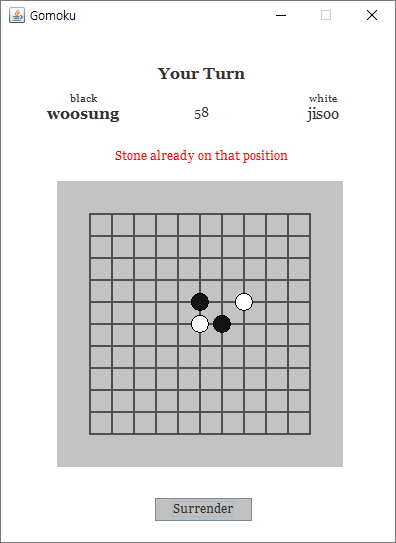
\includegraphics[width=.9\linewidth]{resource/already_stone}
    \caption{돌 중복 배치}
    \label{fig:draw}
  \end{subfigure}
  \caption{게임 부적절 플레이 결과 화면들}
\end{figure}

또한, 보드 밖 영역에 2번 이상 돌을 놓은 경우와 상대방의 연결이 끊긴 경우, 상대방이 항복한
경우, 60초 시간제한을 넘기는 등 예외적인 상황에서도 아래와 같이 제대로 결과가 나타났다.
\begin{figure}[h]
  \centering
  \begin{subfigure}{.24\textwidth}
    \centering
    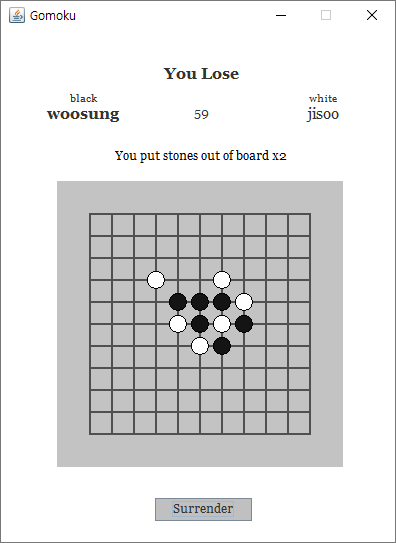
\includegraphics[width=.9\linewidth]{resource/out_of_board2}
    \caption{두 번 보드밖 배치 패배}
    \label{fig:out_of_board2}
  \end{subfigure}
  \begin{subfigure}{.24\textwidth}
    \centering
    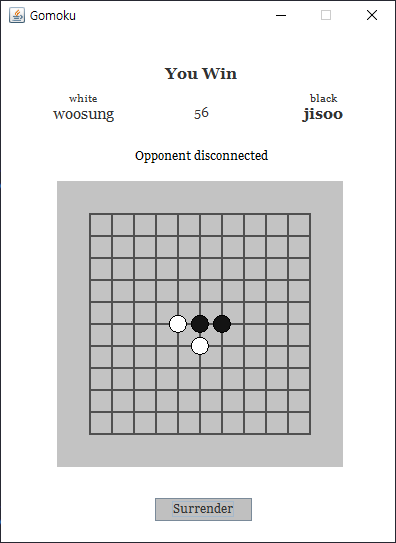
\includegraphics[width=.9\linewidth]{resource/disconnected}
    \caption{상대 연결이 끊겨 승리}
    \label{fig:win}
  \end{subfigure}
  \begin{subfigure}{.24\textwidth}
    \centering
    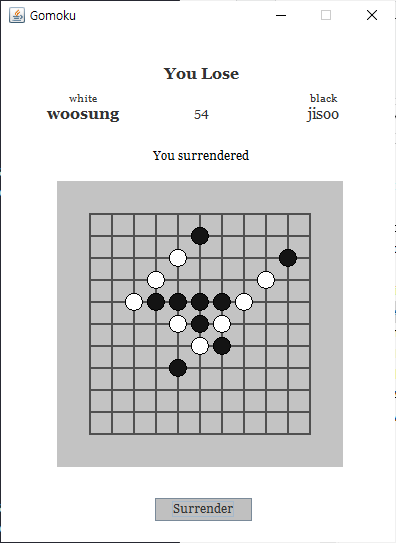
\includegraphics[width=.9\linewidth]{resource/surrender}
    \caption{상대 항복 승리}
    \label{fig:draw}
  \end{subfigure}
  \begin{subfigure}{.24\textwidth}
    \centering
    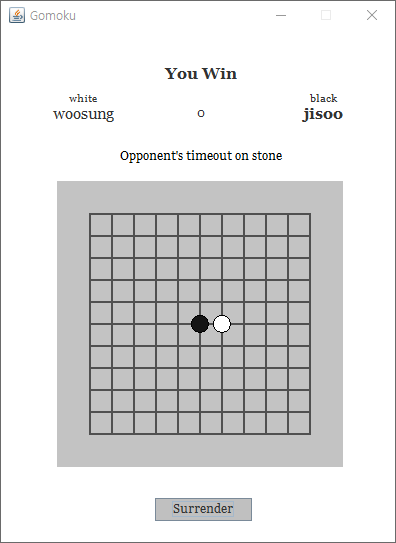
\includegraphics[width=.9\linewidth]{resource/stone_timeout}
    \caption{상대 시간초과 승리}
    \label{fig:draw}
  \end{subfigure}
  \caption{게임 예외 결과 화면들}
\end{figure}
\newpage

\section{Discussion}
\subsection{Thread Based Asynchronous Server}
쓰레드 기반 비동기 서버를 짰다. 때문에 모든 신호들이 새치기를 하며 들어올 수도
있다는 가정을 가지고 FSM을 고안하여 코드를 설계해야했다. 코드 구현이 다소
까다로웠지만, 여러 에러 상황에 더 강한 코드를 작성할 수 있게 된 것 같다.
접두어에 따라 신호를 분류하여 전달하고, 플레이어와 상대방 상태를 따로 관리하였기
때문에 모듈의 역할이 명확하게 세분화되고 가독성이 좋아졌다.

\subsection{Protocol}
어플리케이션 레이어 차원에서 소켓 프로그래밍을 한다는 점에서 여러 예외 상황들에서
자유로웠던 것 같다. 데이터 링크 레이어, 네트워크 레이어, 전송 레이어에서 프레임
전송 여부 확인과 순서 재배치, 에러 교정 과정을 거쳐주기 때문에 주고받은 데이터그램을
충분히 신뢰할 수 있었다. 다만 그럼에도 불구하고 해결할 수 없는 ``클라이언트와의 연결이
끊기는지 여부 실시간 확인'' 문제를 풀기 위해 고민을 해야했었다. 만약 클라이언트 프로그램
예기치 않게 종료되거나, 클라이언트 측의 네트워크가 끊긴다면 서버는 그걸 알 방법이
전혀 없기 때문이다. 그래서 나는 연결 체크(connection check) 신호를 보내기로
계획했고, 나름 성공적이었던 것 같다.

코드의 가독성을 위해 모든 신호를 직관적인 문자열로 구성했지만, 압축된 방식을 사용하여
신호 전달량을 줄일 수 있었지 않았을까하는 아쉬움이 남긴 하다.

\subsection{User Interface}
처음에는 CUI 기반 클라이언트를 완성한 후, GUI 인터페이스의 각 버튼 입력들을
CUI 커맨드로 매핑시켜 큐에 pend시키는 방식으로 구현하였다. 덕분에 GUI 부분의
코드가 최소한으로 남게되어 작업하기가 편했다. 다소 오래된 Java Swing 라이브러리를
사용하여 창의 크기를 마음대로 조절할 수 없는 등의 아쉬운 점이 남기는 하지만,
그래도 대부분의 사용자 인터페이스는 후회없이 만든 것 같다.


\end{document}
